\chapter{Causal Inference Based Fault Localization for Numerical Software with Bayesian Additive Regression Trees}\label{chap:BART}


\section{Introduction}\label{BARTintro}
\vspace{-2pt}
Bayesian Additive Regression Trees(BART)
The motivation for using BART in statistical fault localization is:
\vspace{-0.2cm}
\begin{itemize}
\item BART can flexibly fit non-linear response surfaces even with a large number of predictors
\item BART does not require the researcher to specify the functional form of the relationship between treatment and outcome. The user only need to input the treatment, confounding variable and the outcome, but not need to provide how these variables are parametrically related. Also, comparing to methods such as propensity score matching and subclassification, BART produces coherent posterior predictions. 
\item The casual inference techniques has been proved to be effective in both coverage based fault localization and value based fault localization. The treatment effect estimated with BART appear to be substantially more accurate than linear regression, and propensity score matching with regression adjustment when the treatment variable is binary. It has potential in estimating failure-causing effect for continuous treatment \cite{}.
\item BART algorithm software is freely available and easy to use \cite{}.
\end{itemize}

The rest of the chapter is organized as follows: we present the background of single regression tree and BART model in Section \ref{BARTbg}; Using BART model to estimate failure-causing effect is described in detail in Section \ref{BARTafce};  we report on its empirical evaluation in Section \ref{BARTevaluation}; related work is surveyed in Section \ref{BARTrelatedwork}; and Section \ref{BARTconclusion} concludes the chapter.

\section{BART Model Algorithm}\label{BARTbg}%what is BART and why BART
The BART model algorithm consists of three pars: a sum of regression trees model, a regularization prior and a fitting algorithm Marcov Chain Mote Carlo (MCMC) 
\subsection{A Single Regression Tree model}\label{IIIA}
Regression tree is one type of decision tree that predicts the value of a target variable based on several input variables. Regression tree handles the situation when the target variable is continuous. Figure \ref{singlergt} shows a single regression tree model. All the interior nodes of a regression tree have decision rules which send the input data set to either left or right side. After the input data set go through the interior nodes and reach the bottom of the tree, the data set is divided into several disjoint subgroup. Each group of data is represent by a leaf node. 

\begin{figure*}[!thpb]
\centering
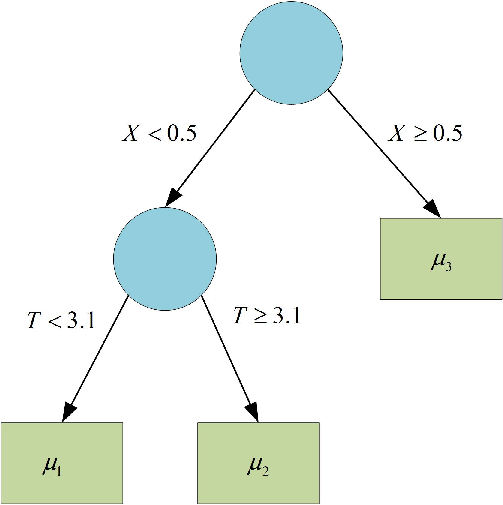
\includegraphics[width=0.5\textwidth]{chapter4_SingleRGT.pdf}
\caption{Single Regression Tree Structure}
\label{singlergt}
\end{figure*}

A single regression tree model is denoted as:
\begin{equation*}
Y=g(\pmb{Z}; R, M)+\epsilon
\end{equation*}
Here $\varepsilon  \sim N(0,{\sigma ^2})$ is a normal distributed error .$\pmb{Z}=[T,\pmb{X}]$ denotes all the variables related to the outcome $Y$, so $Z$ includes both treatment variable $T$ and confounding variables $\pmb{X}$. $R$ denotes a binary regression tree consisting a set of interior node decision rules and a set of terminal nodes, and let $M=
\begin{Bmatrix}
 \mu _1, \mu _2, . . ., \mu _b 
\end{Bmatrix}$
denotes a set of parameter value associated with each of the $b$ terminal nodes of $R$. Each terminal node represent a regression model of outcome $Y$ on all the variables $Z$. 

A regression tree model is often used in approximating unknown functions. For example, if the causal effect of treatment $T$ on outcome $Y$ is decided by an unknown function $Y=f(T,\pmb{X})$, then we can approximate the function $f(T,\pmb{X})$ by fitting a single regression tree model g(\pmb{Z}; R, M) on sample data set. The regression tree model divides the value space of $[T,\pmb{X}]$ in to several subgroups with its tree structure and fit a regression model for each subgroup. When making inference of $Y$ given a specific unit of treatment and confounding variables values $[T=t,\pmb{X}=\pmb{x}]$, the regression will first find out which subgroup the unit belongs to and then infer outcome $Y$ with the corresponding linear regression. Regression tree model has two advantages: (1) making prediction is fast. (2) it can handle non-linear function approximation.


\subsection{A sum of regression trees model}
BART model is a sum of trees model. With the definition of a single tree model, the sum of trees model can be expressed as:
\begin{equation*}
Y = g(\pmb{Z};{R_1},{M_1}) + g(\pmb{Z};{R_1},{M_1}) +  \cdots  + g(\pmb{Z};{R_m},{M_m}) + \varepsilon  
\end{equation*}
where each $(R_i,M_i)$ denotes a single sub-tree model and $\varepsilon  \sim N(0,{\sigma ^2})$.  $m$ denotes the number of trees in BART model. We have
 \begin{equation*}
 Y =f(\pmb{Z})=f(T,\pmb{X})= \left( {\sum\limits_{j = 1}^m {g(T,\pmb{X};{R_j},{M_j})} } \right) + \varepsilon 
 \end{equation*}

Comparing to single regression tree model, BART model has two advantages. First BART is more naturally handle the interaction effects . In the sum of trees model, each tree explains part of the overall fit, so there are many different choices of $(R_1,M_1) \cdots (R_m,M_m)$ can lead to an identical function$ \sum\limits_{j = 1}^m {g(T,\pmb{X};{R_j},{M_j})} $. Second, BART can scale to large datasets using a parallel MCMC sampler \cite{Pratola2015}. Thus, fitting BART model does not has much more computation cost than fitting a large single tree model.  

\subsection{A regularization prior}
Fitting the BART model requires a prior of all the parameters of the sum of trees model.  The prior regularize the fit by keeping the individual tree's effect from being unduly influential. Without such a prior, large  tee components would dominate the sumeof trees structure. The regularization prior can also help BART avoid overfitting. To simplify the prior specification, the trees in BART model $(R_1, M_1), (R_2,M_2), \ldots, (R_m, M_m) $ are considered to be independent of each other and of $\sigma$. Also, the terminal node parameters $ \mu _{1j}, \mu _{2j}, . . ., \mu _{bj} $ of every tree $R_j$ are independent. So we have:

\begin{equation*}
 \begin{array}{l}
P(({R_1},{M_1}),({R_2},{M_2}) \ldots ,({R_m},{M_m}),\sigma ) = \left[ {\prod\limits_j {P({R_j},{M_j})} } \right]p(\sigma )\\
\quad \quad \quad \quad \quad \quad \quad \quad \quad \quad \quad \quad \quad \quad \; = \left[ {\prod\limits_j {P({M_j}|{R_j})P({R_j})} } \right]p(\sigma )
\end{array} 
 \end{equation*}
and
\begin{equation*}
P({M_j}|{R_j}) = \left[ {\prod\limits_i {P({\mu _{ij}}|{R_j})} } \right]
 \end{equation*}
Here ${\mu _{ij}} \in {M_j}$ denotes the $ith$ terminal node of the $jth$ regression tree From the above equations, we can see the independence simplify the prior specification problem to the specification of prior for just ${P({\mu _{ij}}|{R_j})}$, $P({R_j})$ and $P(\sigma)$. In \cite{}, the specification of prior forms on $P(\sigma)$ is defined as the inverse chi-square distribution. The prior on ${P({\mu _{ij}}|{R_j})}$ is defined as conjugate normal distribution. The prior on $P(R_j)$ is complicated which contains 3 aspects: 
\begin{enumerate}
\item the probability that a nonterminal node at depth $d$ is given by 
\begin{equation*}
\alpha {(1 + d)^{ - \beta }},\quad \alpha  \in (0,1),\beta  \in [0,\infty )
 \end{equation*}
\item the prior probability that a variable is selected as the splitting variable at an interior node is $1/k$ and $k$ is the total number of variables including both treatment and confounders. 
\item the prior probability that a splitting variable split at value $x$ is $1/N$ and $N$ is the total number of observed values of the splitting variable in the sample data set.
\end{enumerate}
The detail of the prior specification for ${P({\mu _{ij}}|{R_j})}$, $P({R_j})$ and $P(\sigma)$ can be reffered to \cite{}.


\subsection{Bayesian Backfitting MCMC Algorithm}
BART uses a Bayesian backfitting  MCMC algorithm to fit the model. The algorithm uses Gibbs sampler \cite{}. The Gibbs sampler get $m$ successive draws of $(R_j, M_j)$ conditionally on $(R_{(j)}, M_{(j)}, \sigma)$:

\begin{equation*}
(R_j,M_j)|R_{(j)}, M_{(j)}, \sigma, Y
\end{equation*}
$j=1 \ldots m$, followed by a draw of $\sigma$ from the full conditional: 

\begin{equation*}
\sigma |{R_1}, \ldots ,{R_m},{M_1}, \ldots ,{M_m},Y
\end{equation*}
Here $R_{(j)}$ represents all the trees except $R_j$, so $R_{(j)}$ will be a set of $m-1$ trees. $M_{(j)}$ is similarly defined as $R_{(j)}$. 

\section{BART Model with Causal Inference}\label{BARTafce}% how to use BART

When apply BART model in estimating average causal effects, we use different algorithms for binary treatment and continuous treatment. For binary treatment, BART model primarily estimate failure-causing effects such as $E(Y(1)|\pmb{X}=\pmb{x}) - E(Y(0)|\pmb{X}=\pmb{x})=E(Y|T=1, \pmb{X}=\pmb{x})-E(Y|T=0, \pmb{X}=\pmb{x})=f(1,\pmb(x))-f(0,\pmb(x))$ . The algorithm contains the following steps:
\begin{enumerate}
\item Fit BART model using MCMC algorithm to full sample
\item Get posterior prediction for each unit by setting the treatment variable value $T=1$ and keep confounding variable value unchanged..
\item Get posterior prediction for each unit by setting the treatment variable value $T=0$ and keep confounding variable value unchanged.
\item	Calculate the difference between the posterior predictions for each unit.
\item Estimate failure-causing effect by averaging all the differences of posterior predictions. 
\end{enumerate}

In step 1, the fitted BART model characterized the causal relationship between treatment $T$ and outcome $Y$ given the confounding $\pmb{X}$. We can use the fitted model to predict the outcome $Y$ under different $(T, \pmb{X})$ conditions. For a untreated unit $(T=0, \pmb{X}=\pmb{x})$,  if we set the treatment variable to 1 and then input $(T=1, \pmb{X}=\pmb{x})$ into the BART model, the output is the estimated outcome for that unit in treated condition. Similarly, we can estimate the outcome of a treated unit in untreated condition by inputing $(T=0, \pmb{X}=\pmb{x})$ into the BART model. Thus, in step2, the BART model is used to predict outcome for each unit at observed treatment condition. In step 3, the fitted BART model is used to estimate posterior predictions for each unit at counterfactual condition. Thus, the difference calculated in step 4 is the causal effect estimation for each unit. The average of these differences is failure-causing effect causal effect which is estimated in step 5.

If the treatment variable is continuous, the causal effect of treatment $T$ on outcome $Y$ is characterized by a function $r_e (T)$, which is called dose-response function in medical research. For the failure-causing effect, the dose response functions of continuous treatments are usually non-linear. For example, in Chapter\ref{}, NUMFL use parameterized quadratic model and double linear model to approximate the dose response function within subclasses and get reasonable well result. But the parameterized model has limitations. It usually requires user to make assumptions to specify form of the dose-response function.  For example, in NUMFL, we make some assumptions ($Assumptioin 1, 2, 3$).  The  $Assumptions3$ is: executions with large absolute treatment errors have larger output errors than executions with small values of treatment errors.  Although this assumption is often holds in numeric programs, it is not always to be true. In this case,  the dose response curve of treatment $T$ on outcome $Y$ is likely to deviate from the quadratic model $Y = \zeta {T_e}^2 + \eta {T_e} + c$, which may result in a bad estimation of failure-causing effect. Comparing to parametric model used in NUMFL, BART model does not require user to make assumptions or specify the functional form of the dose response function. The sum of trees structure of BART model can approximate the non-linearity of the DRF during the training phone with MCMC. 

failure-causing effect estimation is a challenge for BART model. In NUMFL, the failure-causing effect is characterized by the coefficient of the regression model.  But in BART model, the sum of trees structure does not such parameters can directly characterize the ACE. To solve this problem, we propose to estimate the treatment causal effect at each unit in the sample. The average of the treatment causal effect on all sample units is the estimated ACE. The causal effect of treatment T on outcome Y for a single unit can be estimated by increasing the treatment variable value of the unit and see how outcome changes. For example, assume a unit $i$ has treatment variable $T=t$ and confounding variables$\pmb {X}=\pmb {x}$, we can use the fitted BART model to estimate the outcome of the unit $Y=y$. Then we increase the treatment variable to $t'=t+\varepsilon$, here $\varepsilon $ is a small number. We input $T'$ and $\pmb{X}$ into the fitted BART model and get the estimated posterior $Y=y'$. Then the estimated causal effect of $T$ on $Y$ for unit $i$ is $\left| {y - y'} \right|$. The algorithm is as follows:
\begin{enumerate}
\item Fit BART model using MCMC algorithm to full sample
\item Increase the treatment variable value $t$ of each unit by $\varepsilon $. The new treatment value $t'=t+\varepsilon$ and the original confounding variables forms a new data set.
\item For each unit, calculate the difference between the posterior prediction in original data set and the posterior prediction in the new data set.
\item Estimate failure-causing effect by averaging all the differences of posterior predictions.
\end{enumerate}

In the above algorithm, the BART model fitted in first step is used to approximate a function $Y=f(T,\pmb(X))$ that specify the dose-response function of the continuous treatment $T$ and confounding variables $\pmb{X}$. Step 2 and Step 3 estimate the treatment causal effect for each sample unit. Step 4 estimate the failure-causing effect of treatment on outcome. 

One problem in step 2 is how to choose the value of the small number $\varepsilon $. But treatment variables in different numerical expressions have different scale of values, it is hard to find a constant $\varepsilon$ which can make $t+\varepsilon$ be a reasonable value for all the treatments. To address this problem, we use the method illustrated by Figure\ref{bartace}.  We sort the original sample data set shown in Figure\ref{bartace} (a) in increasing order according to the value of the treatment variables.  The sorted data set is shown in Figure\ref{bartace} (b). The increased treatment variable value $t'$ in step 2 is equal to the treatment variable value $t$ of the next unit in the list and the last unit in the list will be discarded. Thus, as shown in Figure ref{bartace} (c), for a data set with $n$ observational units, we will have a new data set of $n-1$ units after increasing the treatment variable. The idea behind this method is that we want the value of treatment after increment is a reasonable value that could be observed in  other tests. Also, the value of $t'$ and the value of $t$ are likely to be in the same scale, because they are neighbor in the sorted data set.

\begin{figure*}[!thpb]
\centering
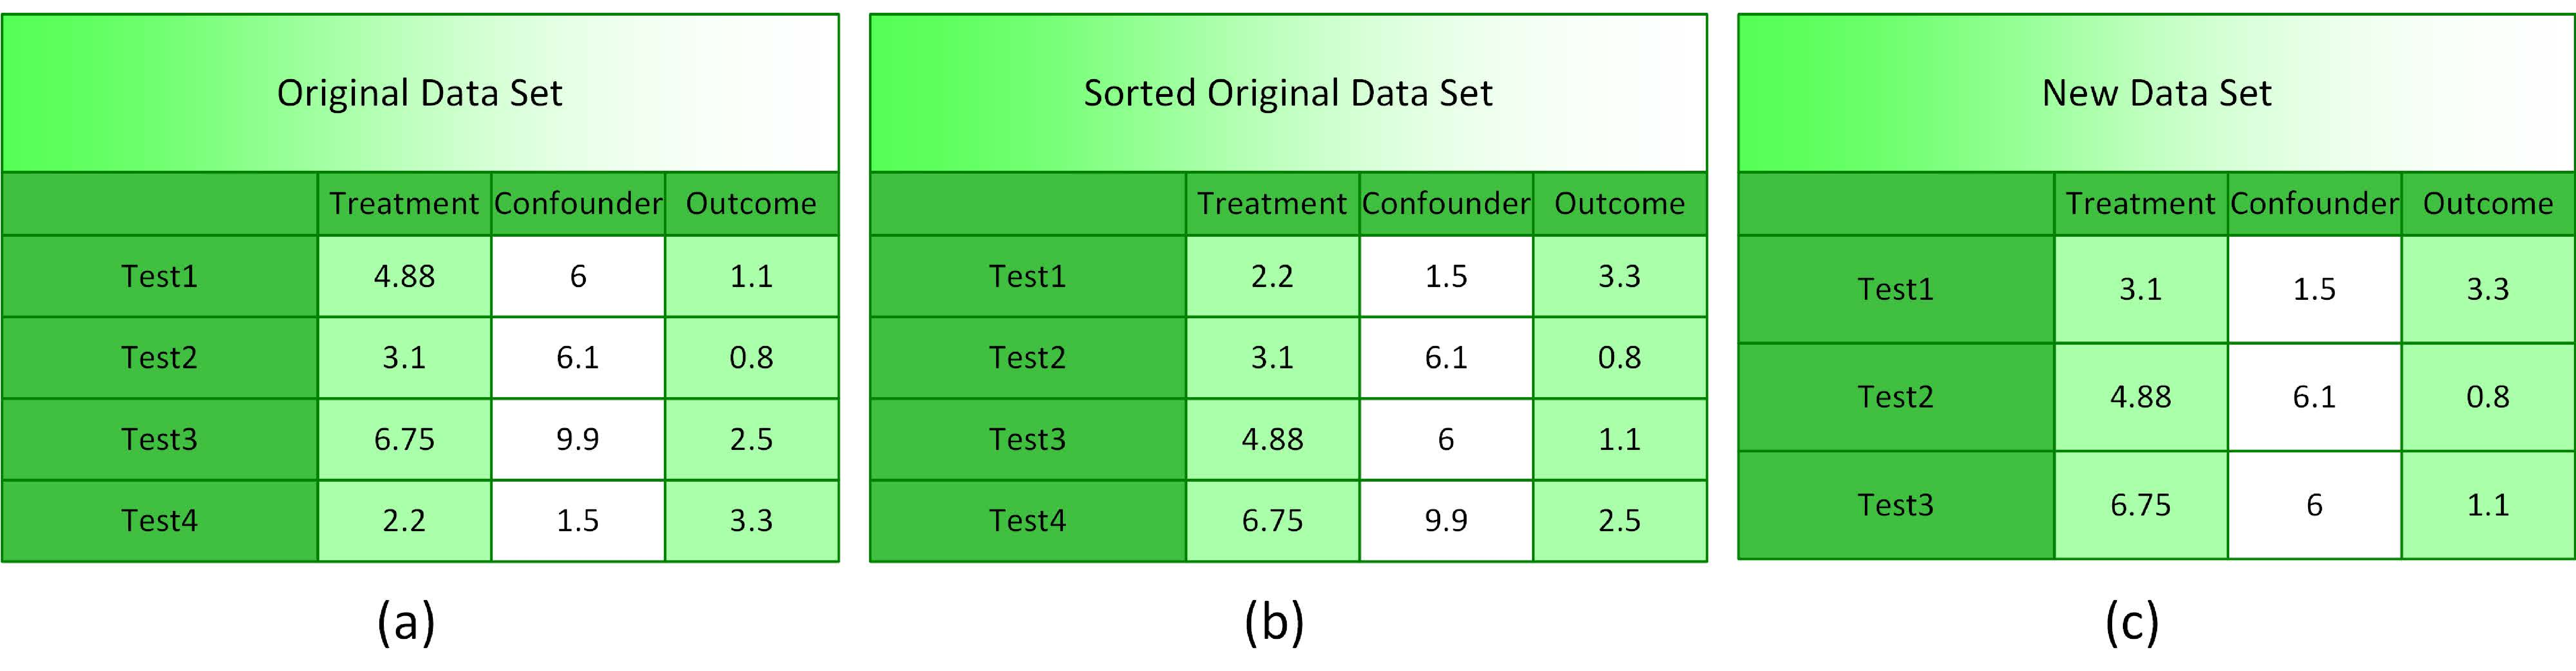
\includegraphics[width=1\textwidth]{chapter4_BART_ACE.pdf}
\caption{EXAMPLE OF TREATMENT VARIABLE INCREAMENT}
\label{bartace}
\end{figure*}

\section{EMPIRICAL EVALUATION}\label{BARTevaluation}% result

To evaluate the effectiveness of BART model, we conducted the empirical study on the same subject programs as described in chapter 3.  The tests suite is also identical to the tests suite in section \ref{numfl_evaluation}.  Overall 92 faulty subject-programs versions with single fault and 25 faulty subject-program versions with two faults. Ochiai, Dstar, SOBER, ESP-SIV are ESP-SCP used as the base line techniques to be compared with BART model. We also compare the performance of BART model with NUMFL-GPS and NUMFL-CBPS which are the proposed in chapter 3. We measured the costs of applying CBPS and the other metrics by the percentage of {\it subexpressions} that need to be examined, in decreasing order of suspiciousness scores, to find the fault, assuming the fault is recognized when it is encountered. 

\subsection{Comparative Performance of BART vs. Baselines}

Figure \ref{QRM_VS_Base} shows the results of comparisons of BART with each of the baseline metrics.  In each graph, the vertical axis represents the percentage improvement (reduction) in cost. The horizontal-axis represents different subject-program versions for which there are cost differences between the metrics, with each version represented by a vertical bar.   Bars above the zero-line represent versions for which BART performed better than the baseline metric and bars below zero represent versions for which BART performed worse.  The length of each bar represents the magnitude of the corresponding cost difference.

\textit{\textbf{ BART vs. Ochiai.}}  Over all 92 faulty subject-program versions, BART performed better than the Ochiai metric on 75 versions but BART performed worse on 17 versions.  There were 41 versions for which BART performed at least 20\% better than the Ochiai metric.  There were just 4 versions for which the latter performed better than BART.

\textit{\textbf{ BART vs. DStar.}}  BART performed better than DStar on 77 subject-program versions but BART performed worse than DStar on 15 versions.  BART performed at least 20\% better than DStar on 44 versions, whereas DStar performed at least 20\% better than BART on just 4 versions.

\textit{\textbf{ BART vs. ESP-SIV.}} BART performed better than ESP-SIV on 78 subject-program versions but BART performed worse than ESP-SIV on 14 versions.  BART performed at least 20\% better than ESP-SIV on 30 versions, whereas ESP-SIV never performed at least 20\% better than BART.

\textit{\textbf{ BART vs. ESP-SCP.}}  BART performed better than ESP-SCP on 75 subject-program versions but BART performed worse than ESP-SCP on 17 versions.  BART performed at least 20\% better than ESP-SIV on 22 versions, whereas ESP-SCP performed at least 20\% better than BART on just 2 versions.

\textit{\textbf{ BART vs. SOBER.}}  BART performed better than SOBER on 73 subject-program versions but BART performed worse than SOBER on 19 versions.  BART performed at least 20\% better than SOBER on 39 versions, whereas SOBER performed at least 20\% better than BART on just 5 versions.

\begin{sidewaysfigure}
\centering
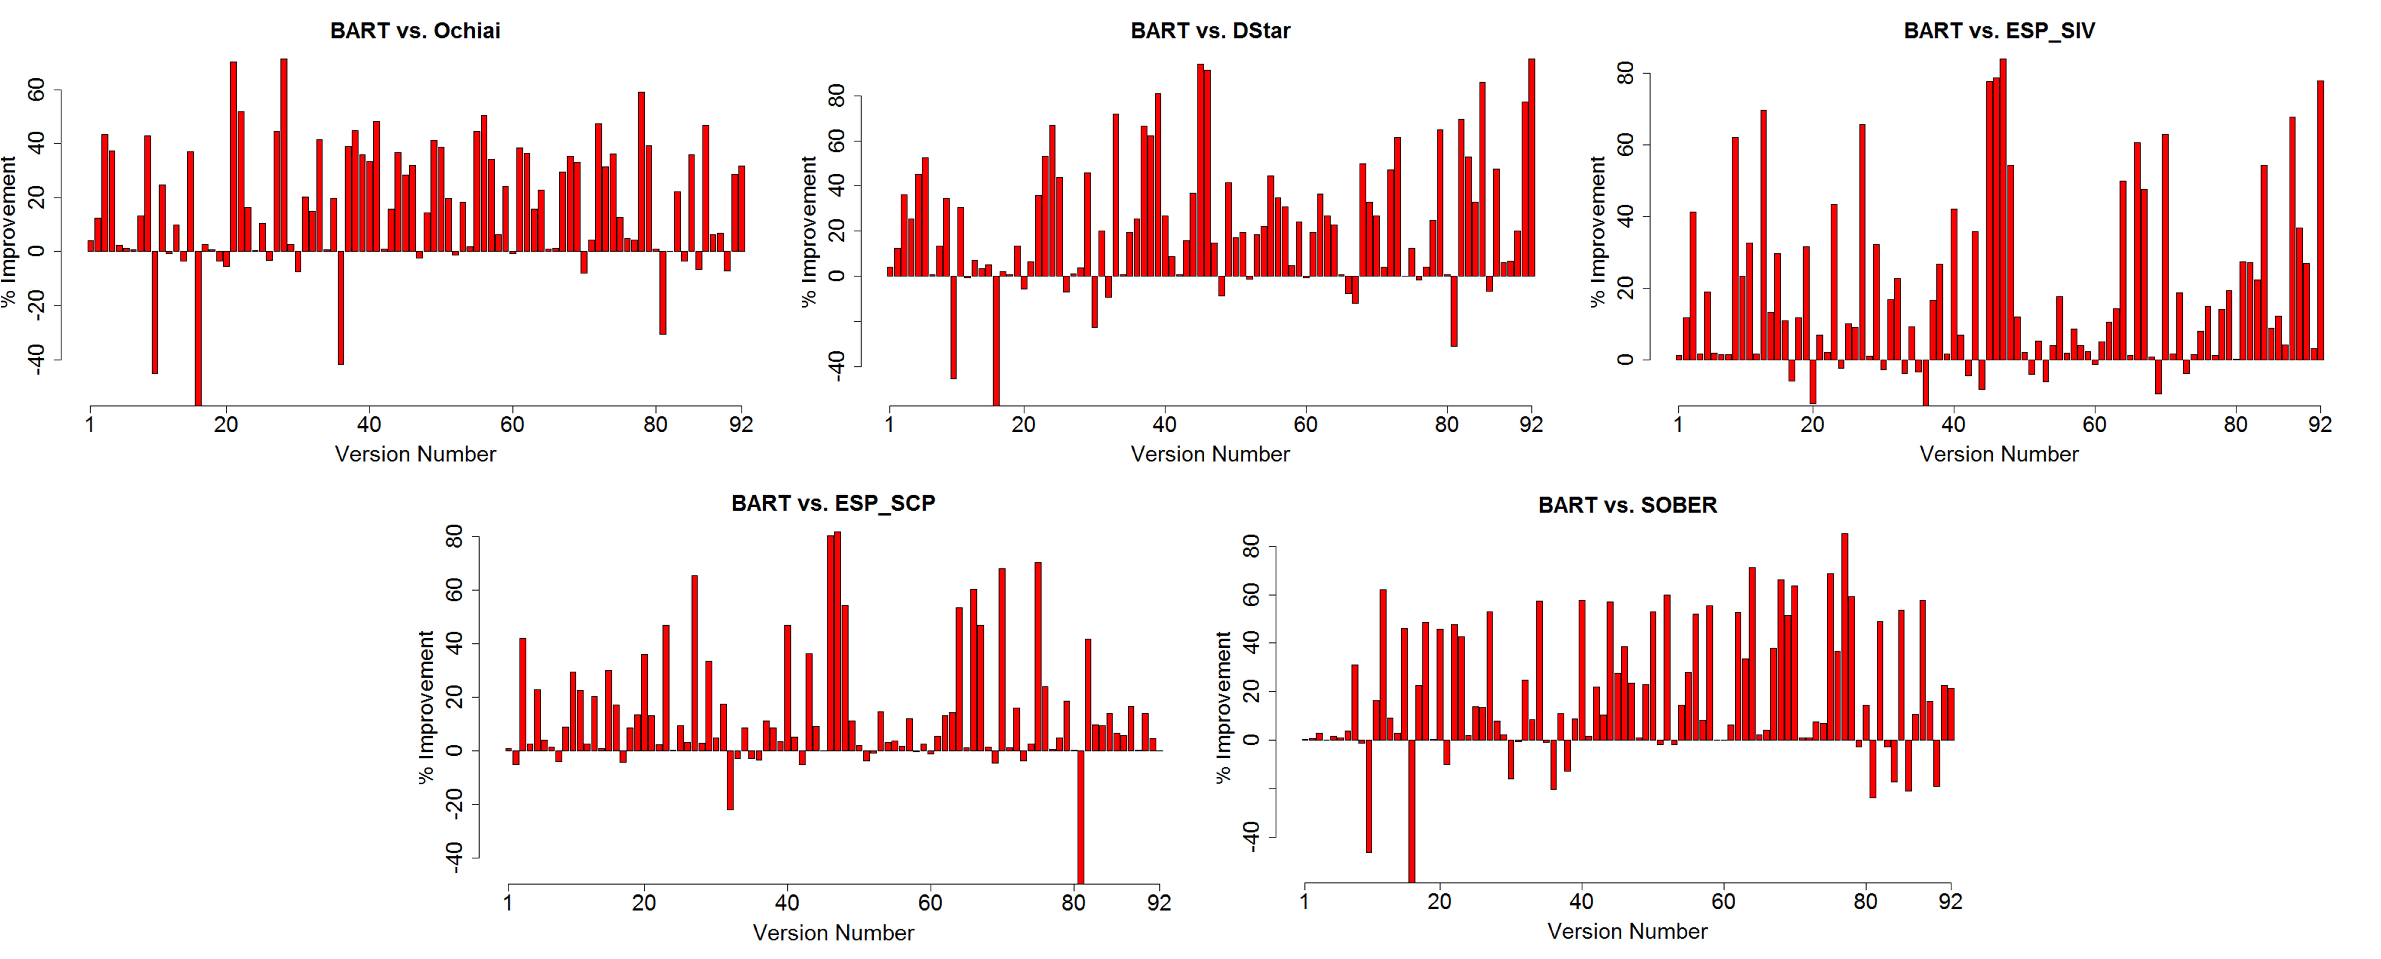
\includegraphics[width=\textwidth]{chapter4_BART_VS_Base.pdf}
\caption{Performance of BART relative to baseline metrics on individual single-fault program versions.}
\label{BART_VS_Base}
\end{sidewaysfigure}

Figure \ref{BART_VS_Base_M} contrasts the performance of BART on the individual two-fault program versions with that of the baseline metrics.  Over all 25 faulty subject-program versions, BART performed better than SOBER on 19 versions but performed worse on 6 versions.  There were 8 versions for which BART performed at least 10\% better than SOBER but 3 versions for which SOBER performed at least 10\% better than BART.  Ochiai performed better than BART on 5 versions but performed worse on 20 versions. BART performed at least 10\% better than Ochiai on 13 versions. BART performed better than both ESP-SIV and ESP-SCP on 20 versions.   BART performed better than DStar on 19 versions.

\begin{sidewaysfigure}
\centering
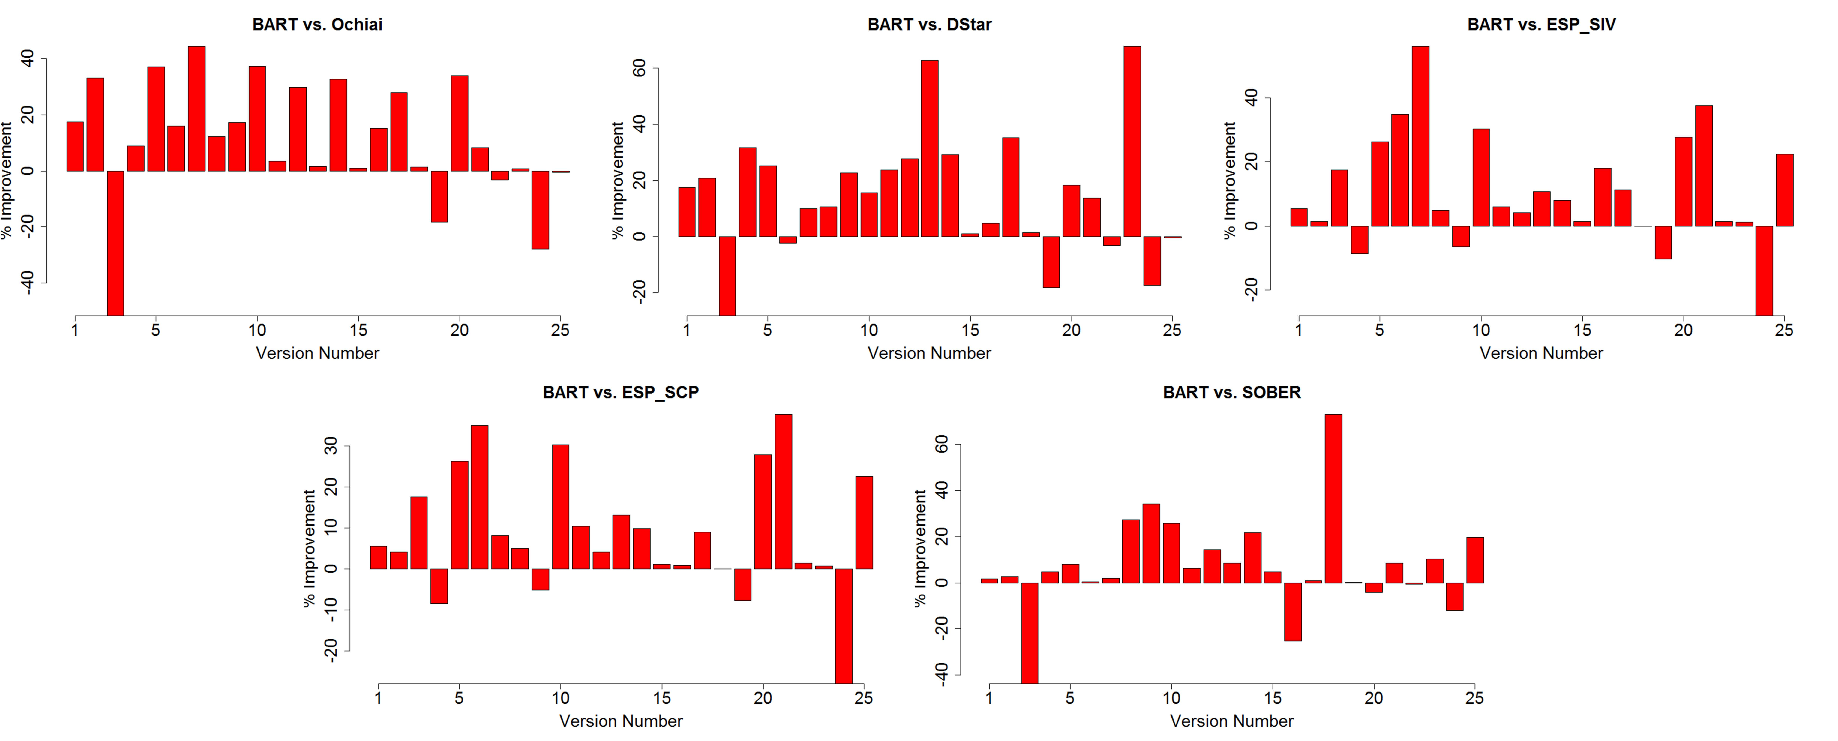
\includegraphics[width=\textwidth]{chapter4_BARTvsBase_M.pdf}
\caption{Performance of BART relative to baseline metrics on individual single-fault program versions.}
\label{BART_VS_Base_M}
\end{sidewaysfigure}


\subsection{BART model vs NUMFL}
Table \ref{tableBARTvsNUMFL} shows the average percentage of subexpressions that had to be examined to find the fault, computed across all the faulty versions, for BART model and NUMFL.  Here we show the results for NUMFL-GPS-QRM and NUMFL-CBPS-QRM.   There were 11 versions for which BART performed better than NUMFL-GPS-QRM. There were 5 versions for which NUMFL-GPS-QRM performed better than BART. BART performed better than NUMFL-CBPS-QRM on 14 versions. There were only 2 versions for which NUMFL-CBPS-QRM performed better than BART. Figure \ref{BARTvsQRM} graphically contrasts the performance of BART and NUMFL-GPS-QRM on the single fault versions.  BART performed better than NUMFL-GPS-QRM on 54 versions, while NUMFL-GPS-QRM performed better on 38 versions.  BART performed at least 20\% better than NUMFL-GPS-QRM on 9 versions, whereas NUMFL-GPS-QRM performed at least 20\% better than BART on 6 versions. Figure \ref{BARTvsCBPS} graphically contrast the performance of BART and NUMFL-CBPS-QRM on the single fault versions.  BART performed better than NUMFL-CBPS-QRM on 61 versions, while NUMFL-CBPS-QRM performed better on 31 versions.  BART performed at least 20\% better than NUMFL-CBPS-QRM on 17 versions, whereas NUMFL-CBPS-QRM performed at least 20\% better than BART on just 4 versions.

\begin{table*}[htbp!]
\caption{AVERAGE FAULT LOCALIZATION COSTS OF BART AND NUMFL METRICS ON SINGLE-FAULT PROGRAM VERSIONS}
\label{tableBARTvsNUMFL}
\centering
      \begin{tabular}{|l|c|c|c|}
      \hline
\multirow{2}{*}{Subject Program}	& \multirow{2}{*}{BART}&	\multicolumn{2}{|c|}{{\bf NUMFL}}	\\	\cline{3-4}
& & GPS-QRM	&CBPS-QRM \\ \hline
Apache\_EigenDecompose &	2.50\%&	12.3\%	&	8.8\%	\\	\hline
Apache\_DScompiler&	9.72\%&	11\%	&	12\%	\\	\hline
Apache\_BigMatrix	&	9.00\%&11.4\%	&	9.9\%	\\	\hline
Apache\_Rotation3D&	9.07\%&	8\%	&	18.9\%	\\	\hline
Ojaljo\_SchurDecompose&	10.61\%&	11.4\%	&	14\%	\\	\hline
Jama\_MatrixDecompose	&11.62\%&	14.2\%	&	23\%	\\	\hline
SciMark\_LU&1.75	\%&	15.3\%	&	27.8\%	\\	\hline
SciMart\_FFT&	37.78\%&	9.5\%	&	19.8\%	\\	\hline
Apache\_SymmLQ&	1.70\%&	2.6\%	&	4.4\%	\\	\hline
Apache\_SplineInterpolator&	4.56\%&	31.7\%	&	35\%	\\	\hline
Apche\_SimpleRegress&	1.24\%&	4.3\%	&	17\%	\\	\hline
Apache\_SchurTransformer&	30.10\%&	3.3\%	&	14.9\%	\\	\hline
Apache\_MillerUpdatRegress&	1.53\%&	7.5\%	&	9.9\%	\\	\hline
Apache\_HarmonicFitter&1.29	\%&	27.3\%	&	32\%	\\	\hline
Apache\_FastSine&	8.33\%&	1.5\%	&	13\%	\\	\hline
Apache\_FastCosine	&	27.59\%&1.3\%	&	1.2\%	\\	\hline
Average Cost	&	10.52\%&10.8\%	&	16.4\%	\\	\hline
\end{tabular}
\end{table*}

\begin{figure*}[!thpb]
\centering
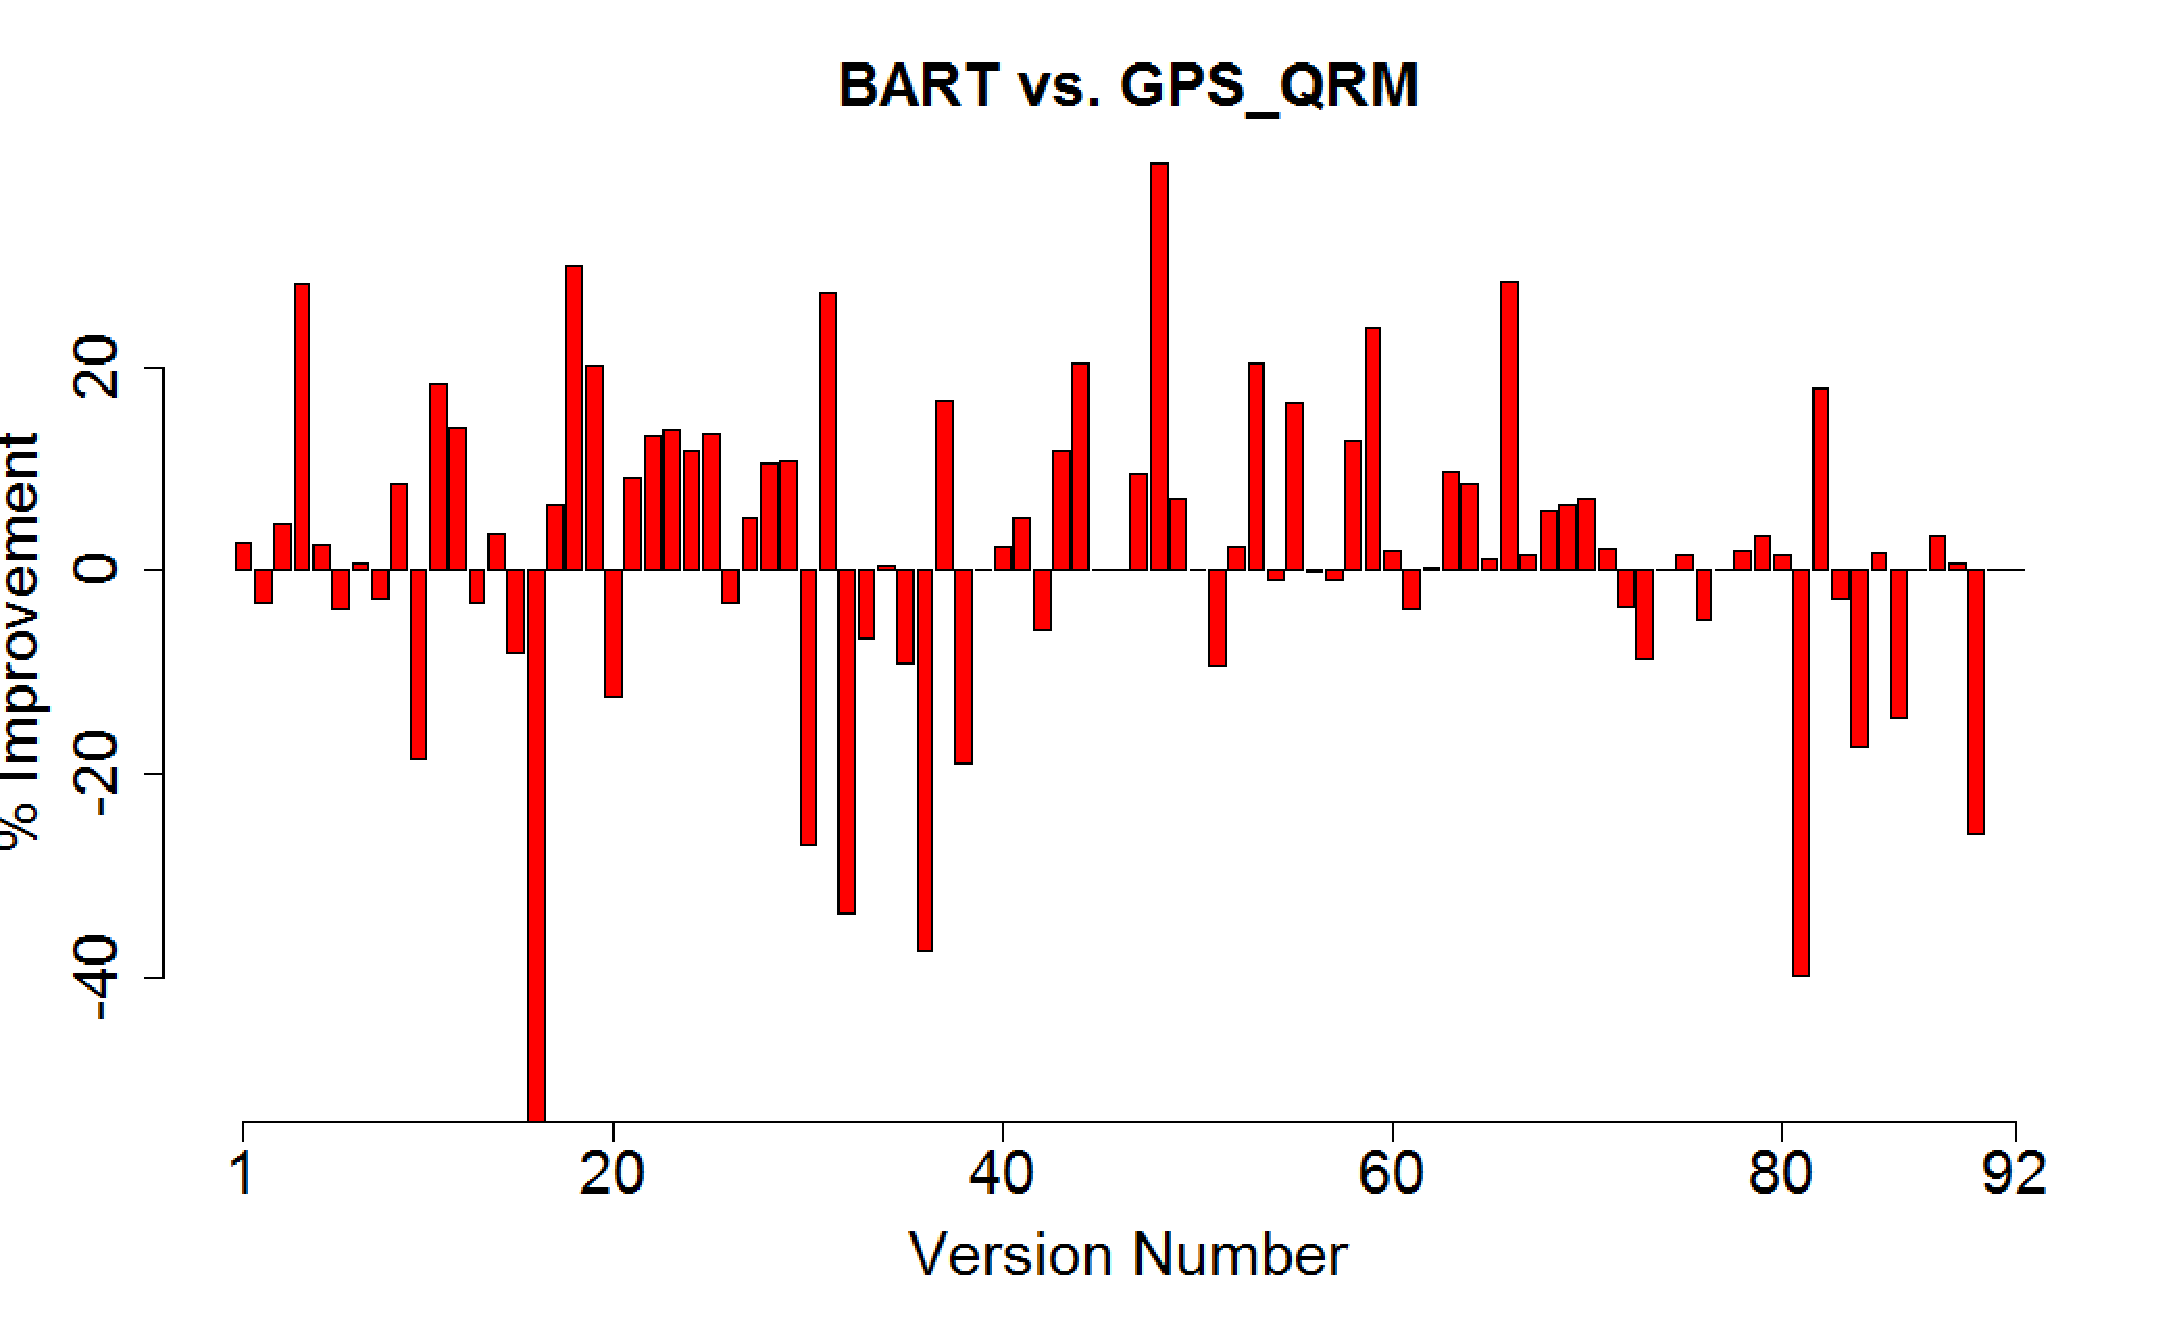
\includegraphics[width=0.8\textwidth]{chapter4_BARTvsGPS_QRM.pdf}
\caption{Relative performance of NUMFL-GPS-QRM with and without data from passing runs, on individual single-fault program versions.}
\label{BARTvsQRM}
\end{figure*}

\begin{figure*}[!thpb]
\centering
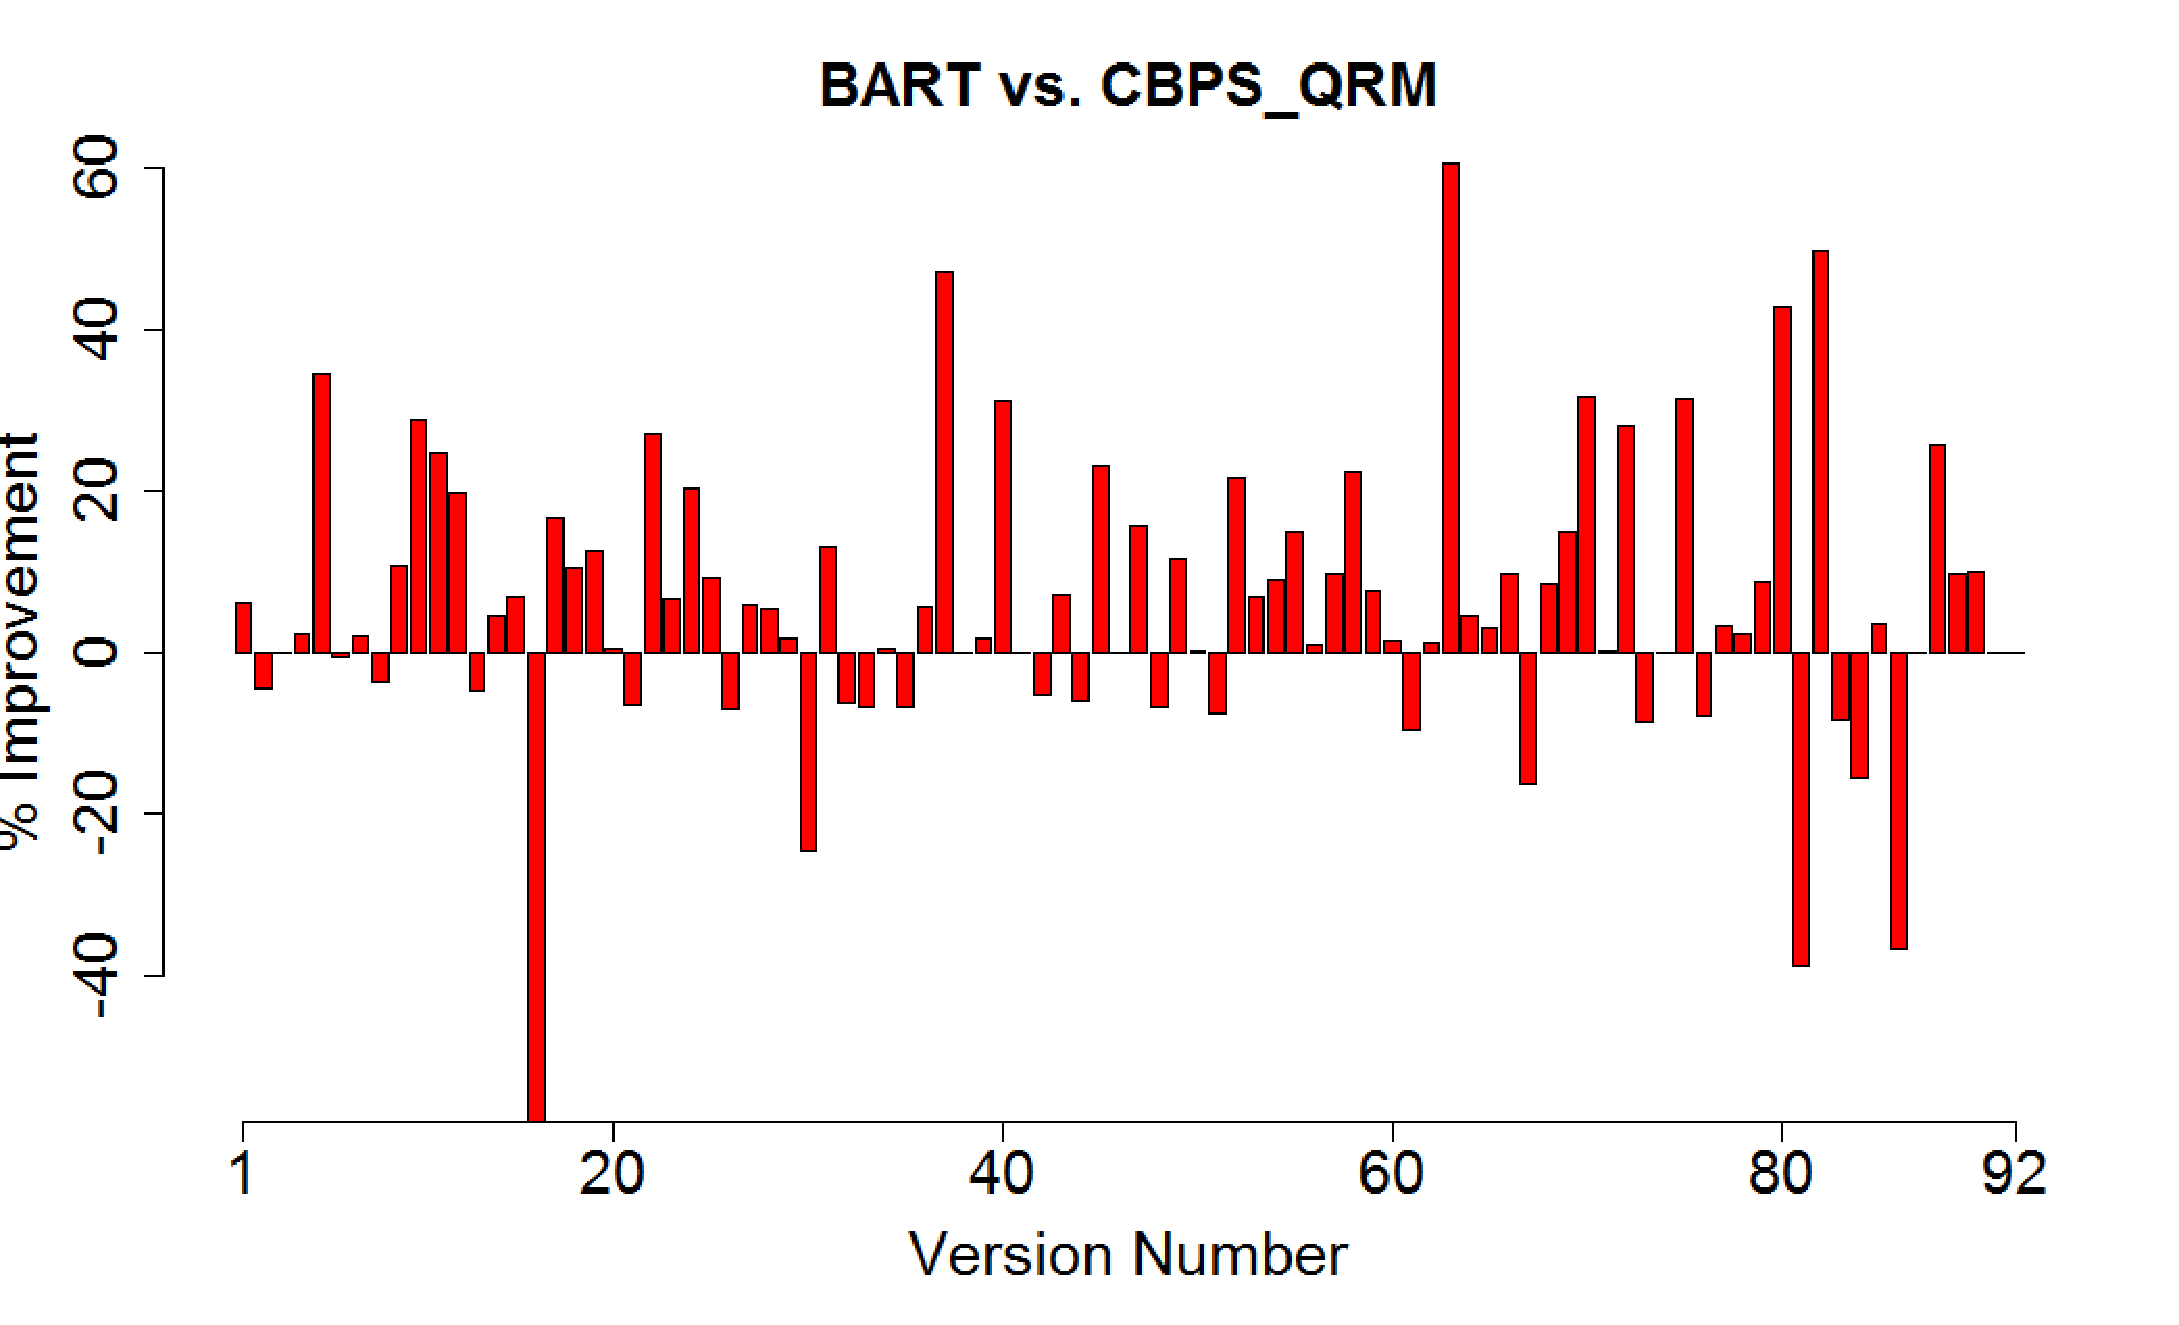
\includegraphics[width=0.8\textwidth]{chapter4_BARTvsCBPS.pdf}
\caption{Relative performance of NUMFL-GPS-QRM with and without data from passing runs, on individual single-fault program versions.}
\label{BARTvsCBPS}
\end{figure*}

Table \ref{table6} shows the average cost, over the faulty versions of each subject program into which two faults were injected, of localizing the first fault to be found, for both NUMFL-GPS-QRM and NUMFL-CBPS-QRM.  NUMFL-GPS-QRM performed better than NUMFL-CBPS-QRM on the two-fault versions of 4 subject programs. NUMFL-GPS-QRM performed worse than NUMFL-CBPS-QRM on the versions of 1 subject program.  Figure \ref{CBPS_VS_GPS_MultipleFault} graphically contrasts the performance of the two methods on the individual two-fault versions.  NUMFL-GPS-QRM performed better than NUMFL-CBPS-QRM on 13 versions and NUMFL-GPS-QRM performed worse on 12 versions.  NUMFL-GPS-QRM performed at least 10\% better than NUMFL-CBPS-QRM on 7 versions, whereas NUMFL-CBPS-QRM performed at least 10\% better than NUMFL-GPS-QRM on just 1 version.

In summary, NUMFL-GPS-QRM performed better than NUMFL-CBPS-QRM on both single-fault and two-fault programs.  The generalized propensity score model $\pmb{\theta}=\pmb{X}'\pmb{\beta}$ achieved better covariate balance than the multinomial logistic regression model used with CBPS.  This may be due to the composition of the data collected from our subject program versions.  The performance of NUMFL-CBPS was poorest with versions that had no more than about 150 failing executions.  However, although NUMFL-CBPS performed worse than NUMFL-GPS in our study, the former's average fault localization cost was still lower than those of the baseline techniques.

\begin{table*}[htbp!]
\caption{AVERAGE FAULT LOCALIZATION COSTS OF NUMFL-GPS-QRM AND NUMFL-CBPS-QRM ON MULTIPLE-FAULT PROGRAM VERSIONS}
\label{table6}
\centering
      \begin{tabular}{|l|c|c|c|}
      \hline
\multirow{2}{*}{Subject Program}	& \multirow{2}{*}{BART}&	\multicolumn{2}{|c|}{{\bf NUMFL}}	\\	\cline{3-4}
& & GPS-QRM	&CBPS-QRM \\ \hline
Apache\_EigenDecompose	&7.98	\%&10.3\%	&	11.1\%	\\	\hline
Apache\_DScompiler	&	5.13\%&4.5\%	&	5.9\%	\\	\hline
Apache\_Rotation3D	&	10.69\%&7.0\%	&	3.0\%	\\	\hline
Ojaljo\_SchurDecompose	&17.55	\%&5.4\%	&	19.8\%	\\	\hline
Jama\_MatrixDecompose	&	4.65\%&14.1\%	&	23.4\%	\\	\hline
{\bf Average Cost} &9.20\% &8.26\% &12.64\%\\ \hline
\end{tabular}
\end{table*}

\begin{figure*}[!thpb]
\centering
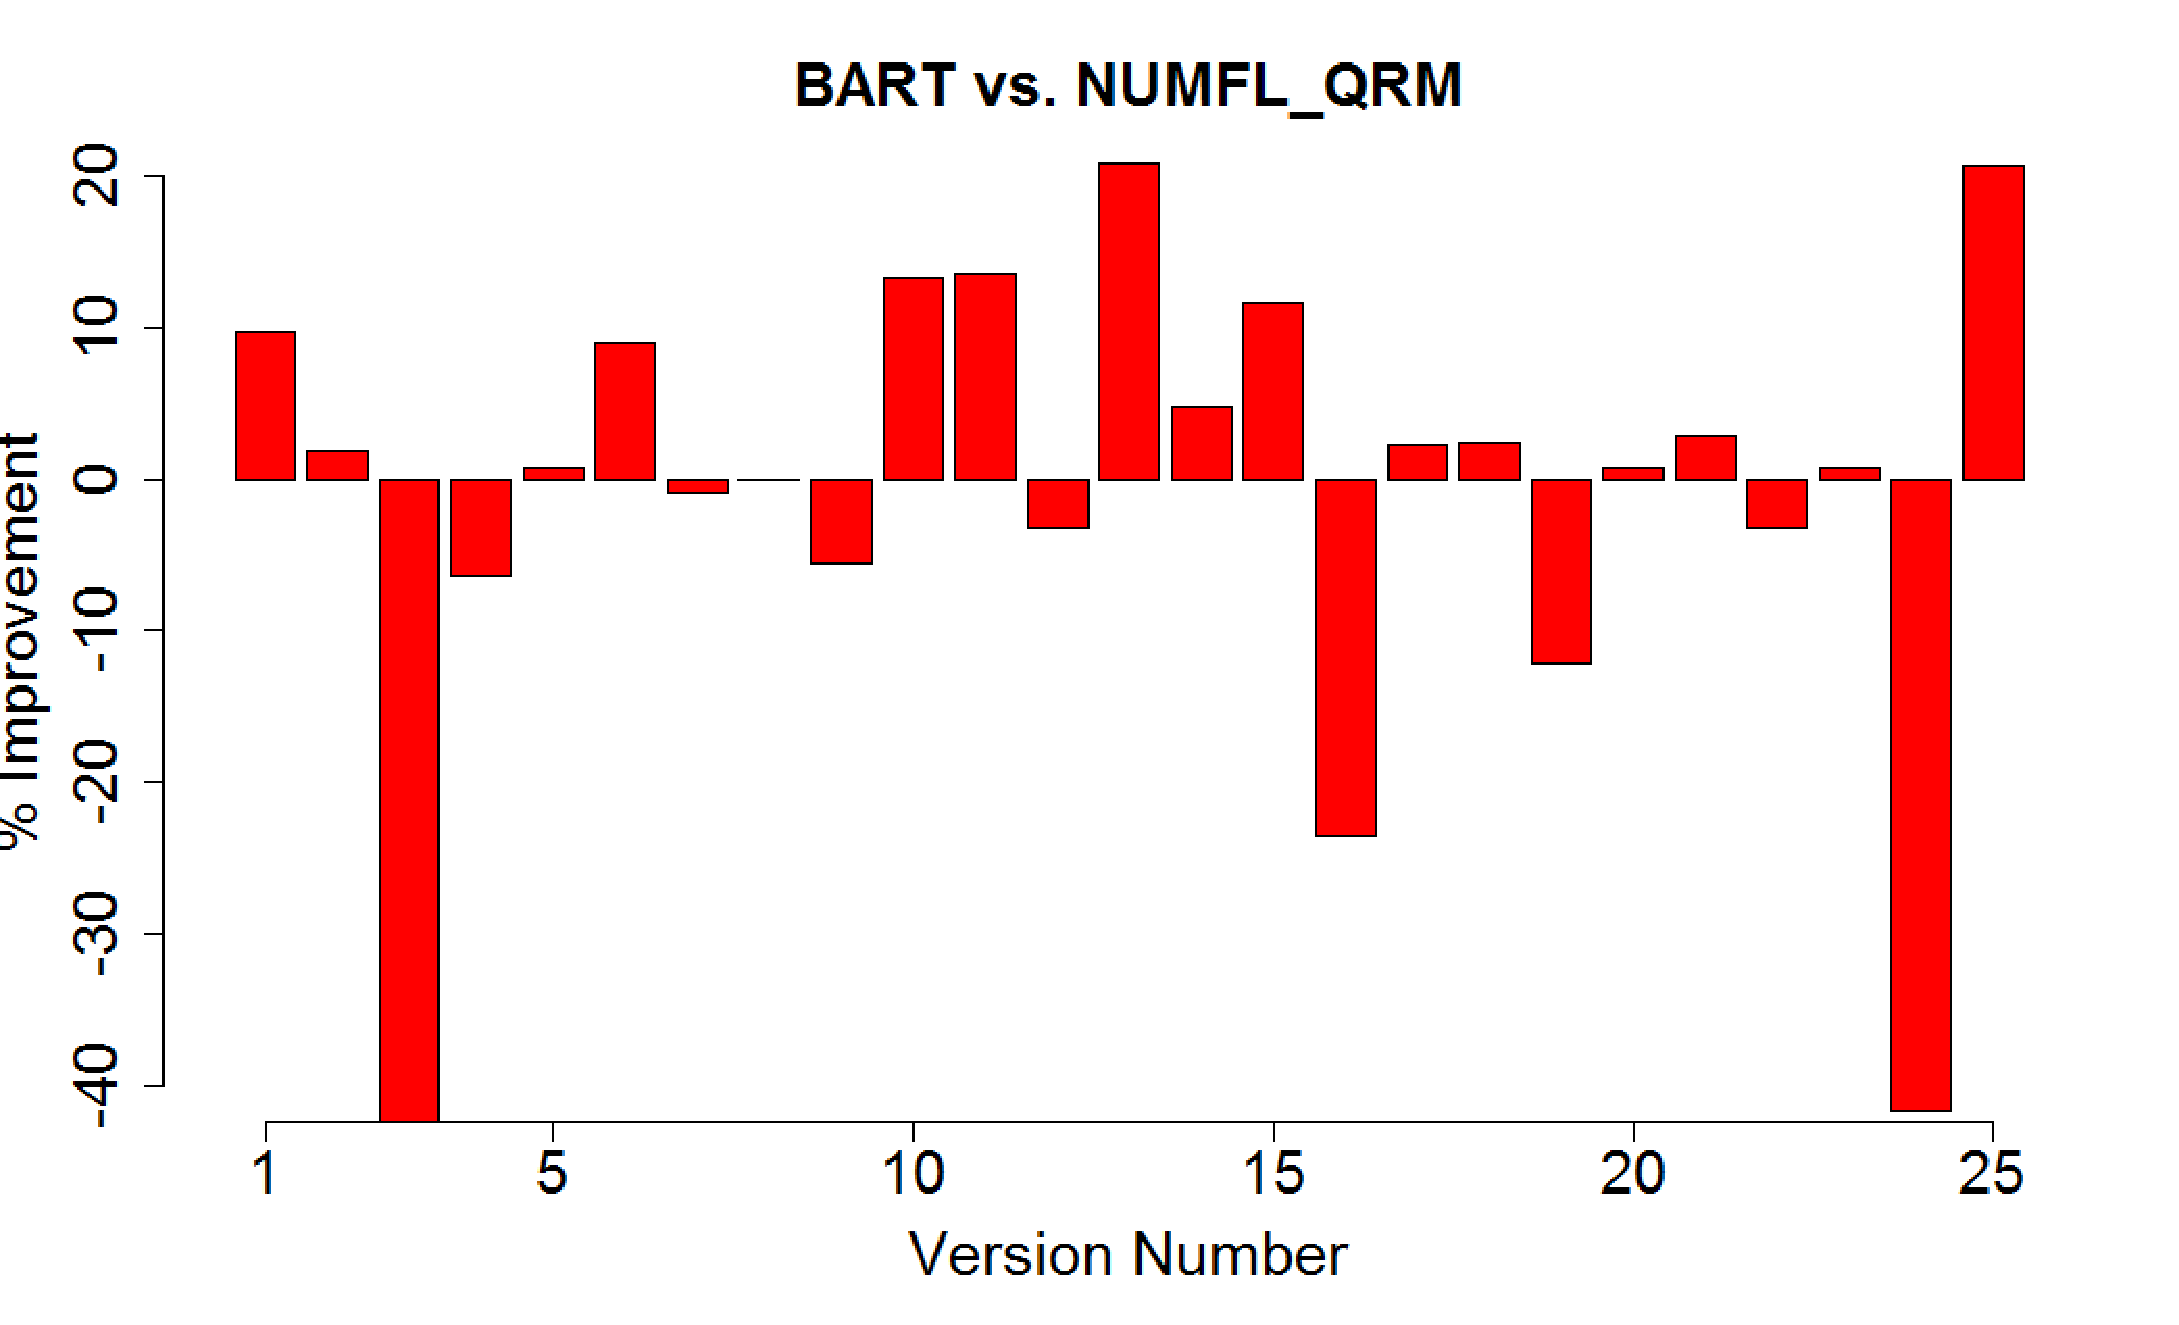
\includegraphics[width=0.8\textwidth]{chapter4_BARTvsGPS_QRM_M.pdf}
\caption{Relative performance of NUMFL-GPS-QRM with and without data from passing runs, on individual single-fault program versions.}
\label{BARTvsGPS_M}
\end{figure*}

\begin{figure*}[!thpb]
\centering
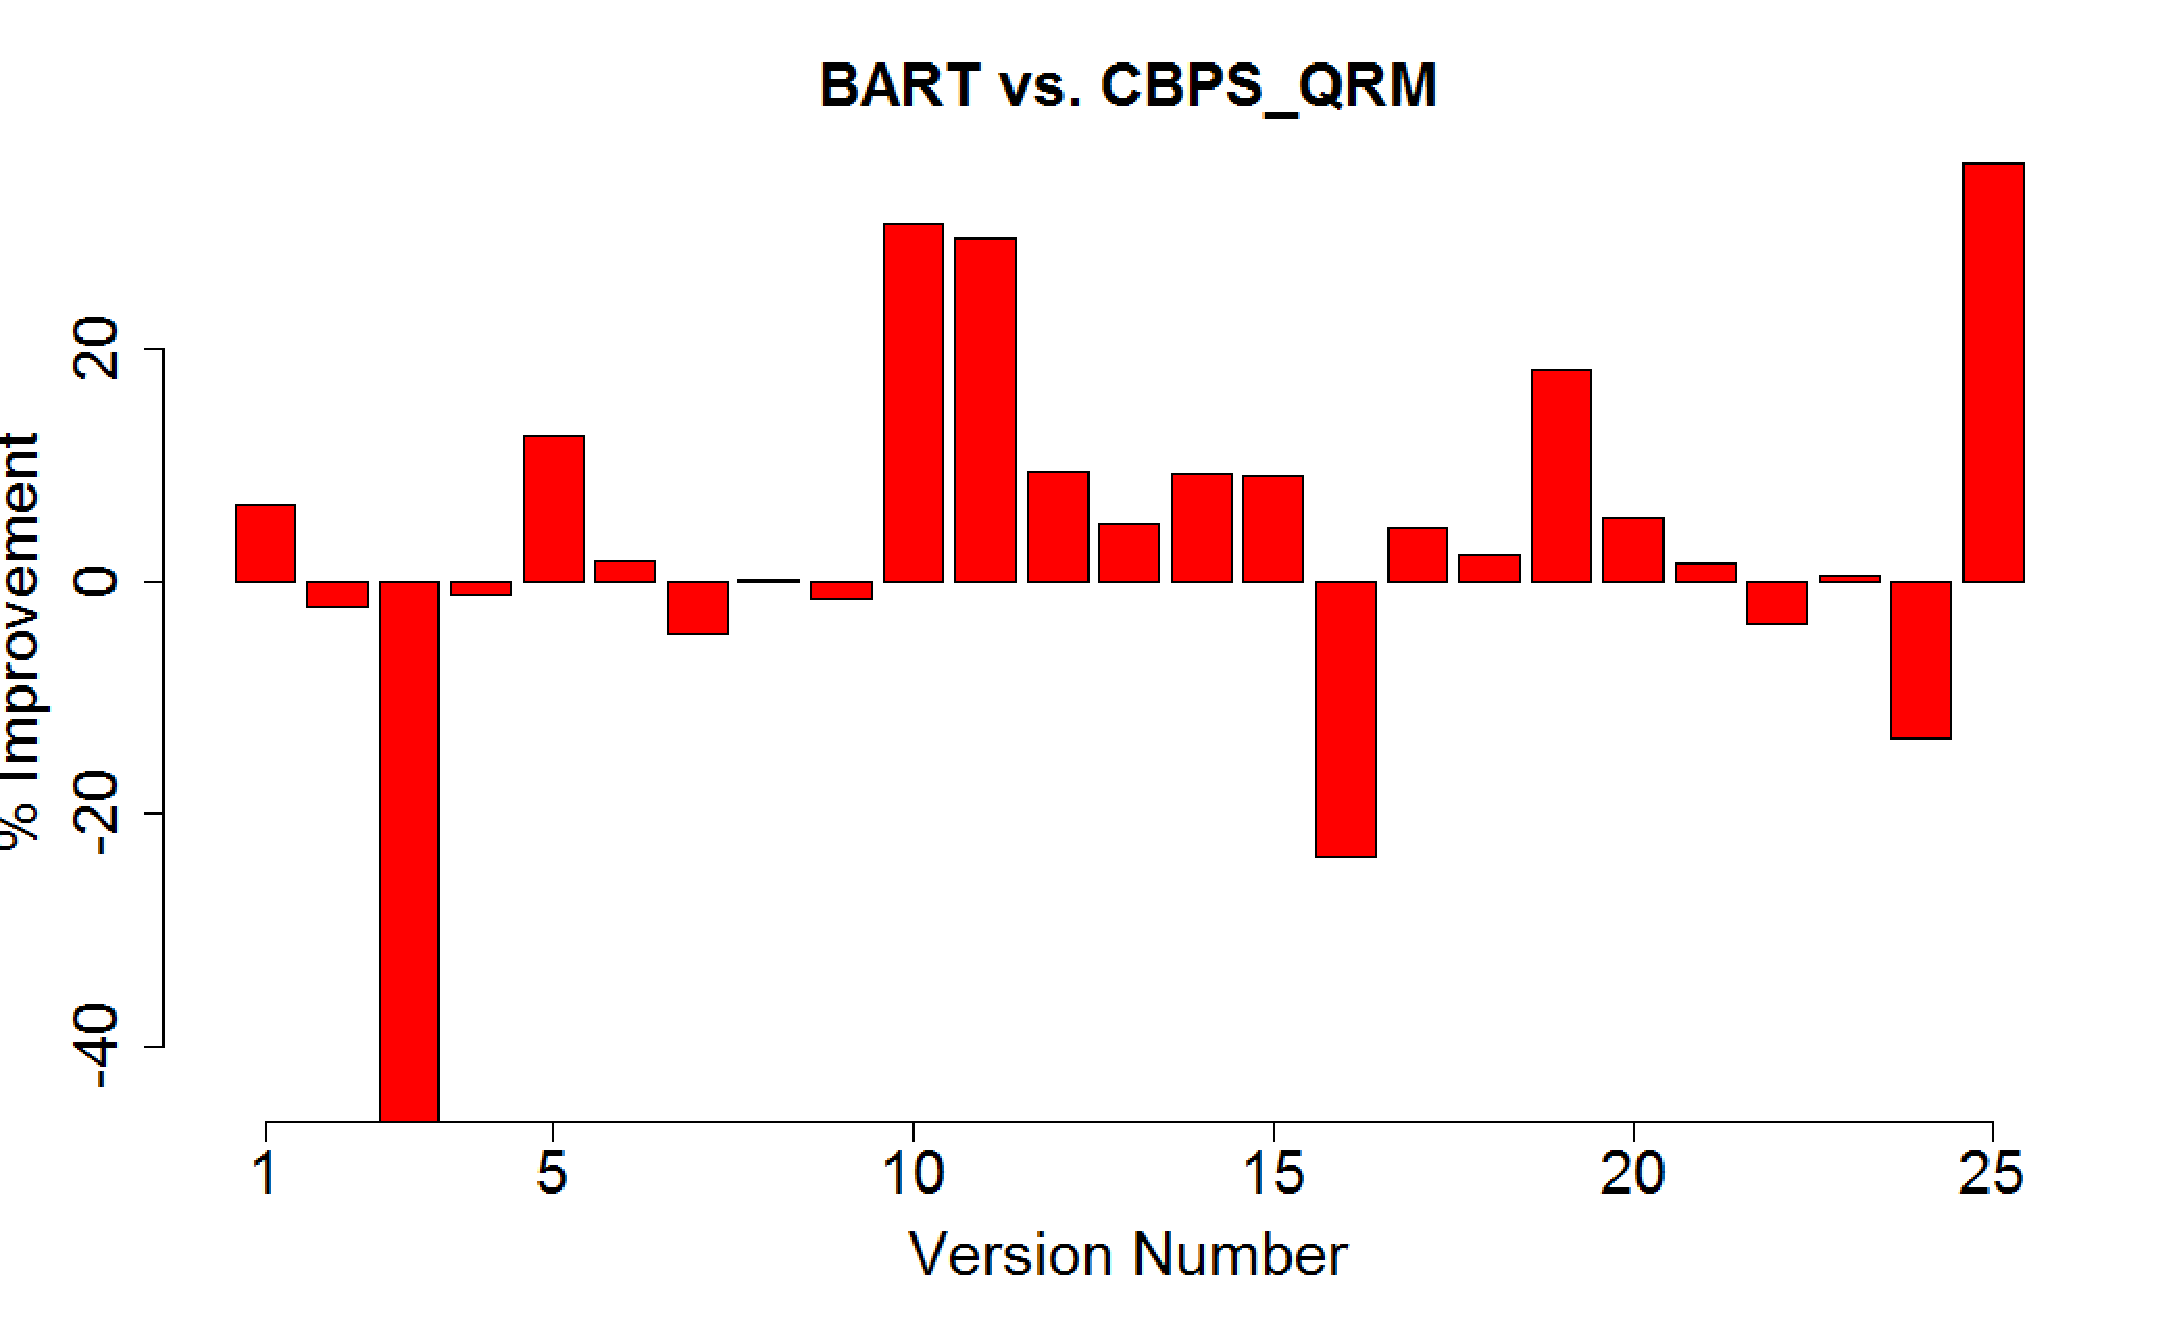
\includegraphics[width=0.8\textwidth]{chapter4_BARTvsCBPS_M.pdf}
\caption{Relative performance of NUMFL-GPS-QRM with and without data from passing runs, on individual single-fault program versions.}
\label{BARTvsCBPS_M}
\end{figure*}

\subsection{Computation Time}
We used two machines for this study: (1) a Dell Precision T5600 with two 2.30 GHz intel Xeon CPUs and 64 GB RAM; and (2) a Dell PowerEdge T300 with a 2.83 GHz Intel Xeon CPU and 24GB RAM. The computation time required to apply any of the non-causal baseline techniques was less than 1 minute per program version. The computation time for NUMFL-QRM and NUMFL-CBPS per version are summarized in table \ref{computetime}

\begin{table*}[htbp!]
\caption{AVERAGE COMPUTATION TIME OF NUMFL-GPS-QRM AND NUMFL-CBPS-QRM ON ONE SINGLE-FAULT PROGRAM VERSIONS }
\label{computetime}
\centering
      \begin{tabular}{|l|c|c|}
      \hline
\multirow{2}{*}{{\bf Subject Program}}	&	\multicolumn{2}{|c|}{{\bf NUMFL}}	\\	\cline{2-3}
  &  GPS-QRM(Seconds) &CBPS-QRM (Seconds)\\ \hline
Apache\_EigenDecompose	&	452.32	&	8.8\%	\\	\hline
Apache\_DScompiler	&	104.66	&	12\%	\\	\hline
Apache\_BigMatrix	&	122.98	&	9.9\%	\\	\hline
Apache\_Rotation3D	&	427.53	&	18.9\%	\\	\hline
Ojaljo\_SchurDecompose	&	463.44	&	14\%	\\	\hline
Jama\_MatrixDecompose	&	403.72	&	23\%	\\	\hline
SciMark\_LU	&	24.72	&	27.8\%	\\	\hline
SciMart\_FFT	&	38.20	&	19.8\%	\\	\hline
Apache\_SymmLQ	&	64.98	&	4.4\%	\\	\hline
Apache\_SplineInterpolator	&	31.7	&	35\%	\\	\hline
Apche\_SimpleRegress	&	54.74	&	17\%	\\	\hline
Apache\_SchurTransformer	&	73.62	&	14.9\%	\\	\hline
Apache\_MillerUpdatRegress	&	97.05	&	9.9\%	\\	\hline
Apache\_HarmonicFitter	&	58.94	&	32\%	\\	\hline
Apache\_FastSine	&	46.59	&	13\%	\\	\hline
Apache\_FastCosine	&	72.75	&	1.2\%	\\	\hline
Average Cost	&	85.79	&	16.4\%	\\	\hline
\end{tabular}
\end{table*}

From \ref{computetime}, The NUMFL is mildly slower than baseline techniques. The NUMFL's computation time is between 7 minutes and 8 minutes for large subject programs and is between  20 seconds to 100 seconds for small subject programs. It is important to mention that we did not attempt to parallelize the computation of AFCE estimates, even though AFCE estimates for different sub-expression can be computed independently.

\section{RELATED WORK}\label{BARTrelatedwork}
The most related works to this study are those using BART model to estimate treatment causal effect. Hill et al. proposed to apply BART model for causal inference and data science \cite{}. In the paper, they designed the method of using BART to estimate average causal effect of binary treatment variable and discussed how to use BART to handle continuous treatment variables and outcome missing data. 

Another related work is using tree structure in fault localization. Chen et al \cite{} present a decision tree learning approach to identify the causes of failures in internet sites. Francis et al \cite{} use tree based method to classify software failures. Kiciman et al \cite{} use decision tree to diagnose which component of large scale systems is the root cause of failure. However, unlike our models, all their works do not localize the fault on statement level.

\section{CONCLUSION}\label{BARTconclusion}
BART model is a Bayesian non-parametric model which can capture both nonlinearities and interactions between variables without knowing the information about how these variables are parametrically related . BART uses a sum of trees structure to approximate the dose response function of continuous treatment variables. The AFCE can be estimated by averaging the causal effect of treatment on outcome at each observation unit. We reported the result of an empirical comparison of BART model to several competing fault localization metrics on both single-fault subject programs and multiple-fault subject programs. BART model performed significantly better than the other techniques. We also compare the BART model with NUMFL, which is introduced in chapter 3. The result shows BART model outperforms NUMFL on single faults localization. In multiple faults localization, BART and NUMFL has similar performances.  We also study the sensitivity of the BART model to the number of trees and the training sample size. The result shows BART is robust on the sample size and number of trees.  In the future work, will seek to extend BART model to localize faults in non numerical softwares with statement coverage or predicate information. 